\documentclass{standalone}
\usepackage{tikz}
\usetikzlibrary{arrows.meta, positioning}

\begin{document}
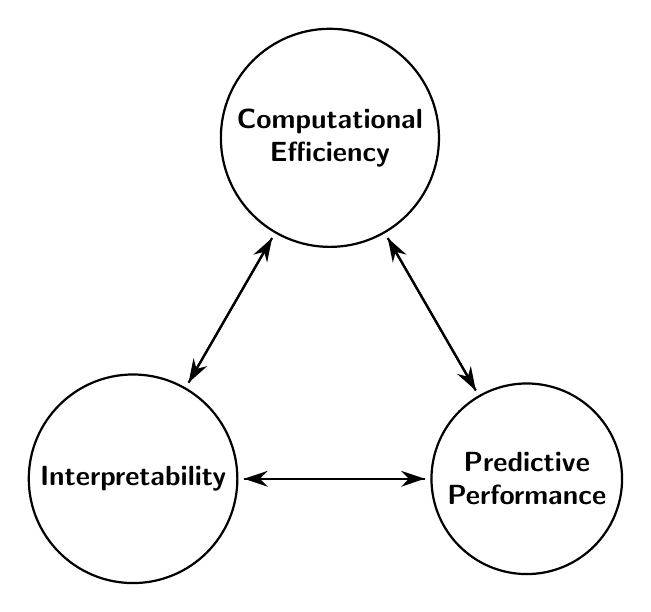
\begin{tikzpicture}[
  node distance=5cm,
  concept/.style={circle, draw, thick, minimum size=2cm, align=center, font=\sffamily\bfseries},
  arrow/.style={thick, -{Stealth[length=3mm, width=2mm]}, shorten >=2pt, shorten <=2pt}
  ]

  % Define the three nodes in an equilateral triangle
  \node[concept] (interp) at (0,0) {Interpretability};
  \node[concept] (perf) at (5, 0) {Predictive\\Performance};
  \node[concept] (comp) at (2.5, 4.33) {Computational\\Efficiency};

  % Connect all nodes with symmetric arrows
  \draw[arrow] (interp) -- (perf);
  \draw[arrow] (perf) -- (interp);

  \draw[arrow] (interp) -- (comp);
  \draw[arrow] (comp) -- (interp);

  \draw[arrow] (perf) -- (comp);
  \draw[arrow] (comp) -- (perf);

\end{tikzpicture}
\end{document}
